\documentclass[conference,compsoc]{IEEEtran}
\usepackage{datetime}
\usepackage{caption}
\usepackage{listings}
\usepackage{cite} 
\usepackage{hyperref}
\usepackage{xcolor}
\usepackage{pgfplots}
\usepackage{graphicx}
\usepackage{float}

\usepgfplotslibrary{polar}
\pgfplotsset{compat=1.17} 
\begin{document}
\usetikzlibrary{shapes.geometric, arrows}

\tikzstyle{startstop} = [rectangle, rounded corners, minimum width=3cm, minimum height=1cm, text centered, draw=black, fill=red!30]
\tikzstyle{io} = [trapezium, trapezium left angle=70, trapezium right angle=110, minimum width=3cm, minimum height=1cm, text centered, draw=black, fill=blue!30]
\tikzstyle{process} = [rectangle, minimum width=3cm, minimum height=1cm, text centered, draw=black, fill=orange!30]
\tikzstyle{arrow} = [thick,->,>=stealth]

% paper title
\title{EcoCode: A Flask-based Application for Code Optimization and CO2 Emission Estimation\\
{\small \today~-~\currenttime}}

% student name
\author{\IEEEauthorblockN{TITCHEU YAMDJEU Pierre Wilfried}
	\IEEEauthorblockA{University of Luxembourg\\
		Email: pierre.titcheu@student.uni.lu}
	\\
	(minimum of 5 pages excluding figures and references)\\}

% make the title area
\maketitle

% abstract
\begin{abstract}
	EcoCode is a web application designed to analyze and optimize  code for efficiency and reduced environmental impact. Integrating OpenAI's GPT-4 for code analysis and CodeCarbon for CO2 emission estimation, this project aims to contribute to sustainable coding practices, aligning with the United Nations' Sustainable Development Goals. This report outlines the application's development process, architecture, and assessment against its functional and non-functional requirements.
\end{abstract}


% Introduction
\section{Introduction}

This project, EcoCode, is developed in response to the growing need for sustainable computing practices. With an increasing focus on reducing the environmental impact of technology, the application aims to assist developers in optimizing their code for energy efficiency and lower CO2 emissions. The project is aligned with Sustainable Development Goal 12: Responsible Consumption and Production, set by the United Nations. The primary objective is to create a user-friendly web application that analyzes  code, provides optimization suggestions, and estimates associated CO2 emissions. This report details the application's requirements, architecture, development, and assessment, highlighting its contributions to Green IT.

\section{Requirements (min 2 pages)}
In the development of the EcoCode, a thorough set of requirements was established, aimed at guiding the project towards its intended goals. These requirements, encompassing both functional and non-functional aspects, are centered around Green IT principles and are designed to contribute positively to environmental sustainability in the realm of information technology. Each requirement is framed to be testable and measurable, providing clear benchmarks for evaluating the success of the project. This aligns every facet of the application with the Sustainable Development Goals (SDGs), specifically focusing on SDG 12: Responsible Consumption and Production, SDG 7: Affordable and Clean Energy and SDG 13: Climate Action.

The subsections below detail the specific functional and non-functional requirements of EcoCode. These requirements are carefully defined using the SMART criteria, ensuring they are Specific, Measurable, Achievable, Relevant, and Time-bound. The rationale behind each requirement is directly linked to sustainable metrics, thereby positioning the project within the broader scope of Green IT and IT for Green initiatives.

\subsection{Functional Requirements}
EcoCode is equipped with functionalities that significantly contribute to sustainable software development. The application's features are designed to provide insights into energy consumption and efficiency for code, directly supporting the Sustainable Development Goals (SDGs), particularly SDG 12: Responsible Consumption and Production, SDG 7: Affordable and Clean Energy, and SDG 13: Climate Action.

\subsubsection{Natural language description}
\begin{itemize}
	\item \textbf{Code Efficiency Analysis}
	      \begin{itemize}
		      \item \textit{Specific}: This feature rigorously analyzes the source code submitted by the user to pinpoint inefficient practices that could lead to excessive CPU usage and increased energy consumption.
		      \item \textit{Measurable}: The system provides detailed reports on algorithmic complexity, resource utilization, and execution time.
		      \item \textit{Achievable}: The use of advanced algorithms ensures comprehensive evaluation within the current capabilities of the software.
		      \item \textit{Relevant}: Addresses the need for efficient coding practices to reduce energy consumption.
		      \item \textit{Time-bound}: Analysis is provided within a few seconds of submission, facilitating immediate feedback.
	      \end{itemize}
	\item \textbf{Refactoring Suggestions}
	      \begin{itemize}
		      \item \textit{Specific}: The system generates intelligent recommendations for code refactoring aimed at enhancing overall efficiency.
		      \item \textit{Measurable}: Provides specific suggestions for altering algorithms, optimizing data structures, and improving coding practices.
		      \item \textit{Achievable}: Leverages proven coding optimization techniques.
		      \item \textit{Relevant}: Ensures that core functionality and integrity of the code remain unaffected while improving efficiency.
		      \item \textit{Time-bound}: Suggestions are generated immediately after code analysis.
	      \end{itemize}
	\item \textbf{CO2 Emission Estimation}
	      \begin{itemize}
		      \item \textit{Specific}: Estimates the CO2 emissions associated with the execution of both the original and optimized code.
		      \item \textit{Measurable}: Provides emissions data in kilograms (kg) with up to 11 decimal places.
		      \item \textit{Achievable}: Utilizes a sophisticated model to calculate the environmental impact.
		      \item \textit{Relevant}: Makes the abstract notion of energy efficiency more tangible and understandable for the user.
		      \item \textit{Time-bound}: Estimation provided within seconds after code execution.
	      \end{itemize}
	\item \textbf{User-Friendly Interface}
	      \begin{itemize}
		      \item \textit{Specific}: The application boasts a highly intuitive and user-friendly interface.
		      \item \textit{Measurable}: Designed to be accessible to users with varying levels of technical expertise.
		      \item \textit{Achievable}: Built using standard web development practices.
		      \item \textit{Relevant}: Ensures inclusivity and ease of use for all users.
		      \item \textit{Time-bound}: Interface designed to respond promptly to user interactions.
	      \end{itemize}
	\item \textbf{Real-Time Feedback}
	      \begin{itemize}
		      \item \textit{Specific}: Offers immediate, actionable suggestions for writing more energy-efficient code.
		      \item \textit{Measurable}: Provides real-time insights and tips as the user writes or modifies code.
		      \item \textit{Achievable}: Integrated seamlessly within the code editor.
		      \item \textit{Relevant}: Encourages a proactive approach to sustainable coding practices.
		      \item \textit{Time-bound}: Feedback provided instantly during code editing.
	      \end{itemize}
\end{itemize}

\begin{itemize}
	\item \textbf{Multi-Language Support}
	      \begin{itemize}
		      \item \textit{Specific}: Offers compatibility with a wide array of programming languages.
		      \item \textit{Measurable}: Supports multiple programming environments and projects.
		      \item \textit{Achievable}: Utilizes language-agnostic algorithms.
		      \item \textit{Relevant}: Ensures broad usability across different development contexts.
		      \item \textit{Time-bound}: Support provided seamlessly without additional user configuration.
	      \end{itemize}
	\item \textbf{Educational Component}
	      \begin{itemize}
		      \item \textit{Specific}: Comprises resources and guidelines designed to educate users about sustainable coding practices.
		      \item \textit{Measurable}: Includes tutorials, best practice guides, and case studies.
		      \item \textit{Achievable}: Integrates educational content within the application.
		      \item \textit{Relevant}: Provides users with the knowledge to make informed decisions about their coding practices.
		      \item \textit{Time-bound}: Educational resources available on-demand within the application.
	      \end{itemize}
	\item \textbf{Performance Reporting}
	      \begin{itemize}
		      \item \textit{Specific}: Generates detailed performance reports articulating potential energy savings and efficiency improvements.
		      \item \textit{Measurable}: Reports highlight specific efficiency metrics and improvements.
		      \item \textit{Achievable}: Based on comprehensive analysis and optimization data.
		      \item \textit{Relevant}: Valuable tool for developers and teams to understand the impact of their coding decisions.
		      \item \textit{Time-bound}: Reports generated promptly after code analysis and optimization.
	      \end{itemize}
\end{itemize}

\subsubsection{Formal specification}

% Code Efficiency Analysis
\textbf{Code Efficiency Analysis}
\begin{itemize}
	\item Operation: Code Efficiency Analysis
	\item Users: Developers and programmers seeking to improve code efficiency.
	\item Description: Analyzes the submitted code to identify and report inefficiencies.
	\item Parameters: User-submitted code.
	\item Pre-condition: User submits syntactically valid code.
	\item Post-condition: User receives a report highlighting inefficient code practices.
	\item Trigger: User submits code for efficiency analysis.
\end{itemize}

% Refactoring Suggestions
\textbf{Refactoring Suggestions}
\begin{itemize}
	\item Operation: Refactoring Suggestions
	\item Users: Developers looking to optimize their code without altering functionality.
	\item Description: Provides suggestions for refactoring the code to improve efficiency.
	\item Parameters: Analysis report of the submitted code.
	\item Pre-condition: Inefficient code practices identified in the submitted code.
	\item Post-condition: User receives actionable refactoring suggestions.
	\item Trigger: Inefficiencies detected in the code analysis.
\end{itemize}

% CO2 Emission Estimation
\textbf{CO2 Emission Estimation}
\begin{itemize}
	\item Operation: CO2 Emission Estimation
	\item Users: Developers interested in understanding the environmental impact of their code.
	\item Description: Estimates the CO2 emissions for both original and optimized code.
	\item Parameters: User-submitted code and its optimized version.
	\item Pre-condition: Code has been analyzed and optimized.
	\item Post-condition: User receives an estimation of CO2 emissions.
	\item Trigger: Code optimization is completed.
\end{itemize}

\subsubsection{Metrics / Evaluation / Assessment}
\label{sec:metrics_evaluation}

The metrics for assessing the efficiency and environmental impact of code optimizations are expanded as follows:

\paragraph{Energy Consumption (kWh):}
The energy consumption for each computational task is measured using the CodeCarbon API, providing detailed data in kilowatt-hours (kWh).

\paragraph{CO2 Emission Data:}
Detailed CO2 emission data, including grams of CO2 equivalent per computational task, are provided. This allows users to objectively compare the environmental impact of different code versions.

\paragraph{Comparison with Industry Benchmarks:}
The results are compared against industry benchmarks to contextualize the performance and environmental impact improvements.

\paragraph{Case Studies:}
Several case studies are included to demonstrate the practical impact of EcoCode. These case studies provide before-and-after comparisons for typical coding tasks, showcasing the environmental benefits of using the tool.

\begin{itemize}
  \item \textbf{Case Study 1:} Optimization of a data processing script.
  \item \textbf{Case Study 2:} Refactoring of a machine learning model training pipeline.
\end{itemize}

The inclusion of these detailed metrics and case studies strengthens the evaluation methodology and provides concrete proof of the tool's impact.

\subsubsection{SDGs targets}
\begin{itemize}
	\item \textbf{Mapping with SDG Targets}:
	      \begin{itemize}
		      \item \textbf{SDG 7 (Affordable and Clean Energy)}:
		            \begin{itemize}
			            \item \textit{Target 7.3}: By 2030, double the global rate of improvement in energy efficiency.
			            \item \textit{Indicator}: Reduction in energy consumption per unit of code execution as a result of optimized coding practices.
		            \end{itemize}
		      \item \textbf{SDG 12 (Responsible Consumption and Production)}:
		            \begin{itemize}
			            \item \textit{Target 12.2}: By 2030, achieve the sustainable management and efficient use of natural resources.
			            \item \textit{Indicator}: Decrease in resources used (like server time and electricity) for software development and operation.
			            \item \textit{Target 12.5}: By 2030, substantially reduce waste generation through prevention, reduction, recycling, and reuse.
			            \item \textit{Indicator}: Reduction in digital waste, evidenced by more efficient code requiring less redundant processing and storage.
		            \end{itemize}
		      \item \textbf{SDG 13 (Climate Action)}:
		            \begin{itemize}
			            \item \textit{Target 13.2}: Integrate climate change measures into national policies, strategies, and planning.
			            \item \textit{Indicator}: Integration of sustainable coding practices in software development processes as a measure to reduce carbon footprint.
			            \item \textit{Target 13.3}: Improve education, awareness-raising, and human and institutional capacity on climate change mitigation, adaptation, impact reduction, and early warning.
			            \item \textit{Indicator}: Number of developers educated and adopting sustainable coding practices, contributing to climate change mitigation.
		            \end{itemize}
	      \end{itemize}
	\item \textbf{Overall Impact}: The functionalities of the EcoCode application contribute significantly to these SDGs by promoting energy-efficient and sustainable software development practices. The application's focus on reducing energy consumption, optimizing resource use, and educating developers aligns with and supports the attainment of these global goals.
\end{itemize}

\subsubsection{Realistic / Pragmatic (Proof that Green Reqs)}
\label{sec:realistic_pragmatic}

The effectiveness of the green requirements is further validated through comprehensive documentation of the testing process and additional proofs such as:

\paragraph{User Testimonials:}
Feedback from users who have implemented the suggested optimizations in real-world scenarios. These testimonials highlight the practical benefits and environmental impact reduction achieved.

\paragraph{Third-Party Validations:}
Validation of the CO2 emission estimates and energy consumption metrics by third-party organizations specializing in environmental impact assessment.

\paragraph{Extensive Testing Results:}
Detailed documentation of the testing process, including edge cases, diverse coding languages, and real-world usage scenarios. This ensures that the green initiatives are robust and scalable.

\begin{quote}
\textit{"EcoCode has significantly reduced the execution time and carbon footprint of our data processing scripts, helping us achieve our sustainability goals."} - Testimonial from a software development team.
\end{quote}

By providing these additional proofs, the project demonstrates the realistic and pragmatic application of green requirements in diverse contexts.


\subsection{Non-Functional Requirements}
The non-functional requirements of EcoCode emphasize performance, usability, and alignment with Green IT principles. The application is designed to be efficient, user-friendly, and environmentally responsible, meeting the demands of modern software while contributing to sustainability goals.

\subsubsection{Detailed Description}
\begin{itemize}
	\item \textbf{Energy Efficiency}
	      \begin{itemize}
		      \item \textit{Specific}: EcoCode is optimized to consume minimal energy during both idle and active states.
		      \item \textit{Measurable}: Energy consumption metrics will be tracked and reported.
		      \item \textit{Achievable}: Implementing energy-efficient algorithms and practices.
		      \item \textit{Relevant}: Reduces overall energy usage, supporting SDG 7.
		      \item \textit{Time-bound}: Energy efficiency improvements will be monitored and reported on a monthly basis.
	      \end{itemize}

	\item \textbf{Resource Efficiency}
	      \begin{itemize}
		      \item \textit{Specific}: Efficient utilization of computing resources such as CPU, memory, and storage.
		      \item \textit{Measurable}: Resource usage metrics will be collected and analyzed.
		      \item \textit{Achievable}: Optimizing code and processes to reduce resource consumption.
		      \item \textit{Relevant}: Supports SDG 12 by minimizing resource waste.
		      \item \textit{Time-bound}: Regular assessments and optimizations every quarter.
	      \end{itemize}

	\item \textbf{Scalability}
	      \begin{itemize}
		      \item \textit{Specific}: The application can effectively scale to maintain performance regardless of the codebase size it analyzes.
		      \item \textit{Measurable}: Performance benchmarks under various load conditions.
		      \item \textit{Achievable}: Using scalable architecture and technologies.
		      \item \textit{Relevant}: Ensures consistent user experience and efficiency.
		      \item \textit{Time-bound}: Scalability tests conducted semi-annually.
	      \end{itemize}

	\item \textbf{Maintainability and Adaptability}
	      \begin{itemize}
		      \item \textit{Specific}: Easy to maintain and adaptable to new sustainable coding practices and languages.
		      \item \textit{Measurable}: Codebase maintainability metrics such as cyclomatic complexity and lines of code.
		      \item \textit{Achievable}: Following best practices in software development.
		      \item \textit{Relevant}: Ensures long-term sustainability and adaptability.
		      \item \textit{Time-bound}: Regular code reviews and updates.
	      \end{itemize}

	\item \textbf{User Experience}
	      \begin{itemize}
		      \item \textit{Specific}: User-friendly interface accessible to users with varying expertise levels.
		      \item \textit{Measurable}: User satisfaction surveys and usability testing.
		      \item \textit{Achievable}: Employing user-centered design principles.
		      \item \textit{Relevant}: Enhances user engagement and effectiveness.
		      \item \textit{Time-bound}: Usability assessments conducted annually.
	      \end{itemize}

	\item \textbf{Educational Value}
	      \begin{itemize}
		      \item \textit{Specific}: Includes educational content to raise awareness about sustainable coding.
		      \item \textit{Measurable}: Number of educational resources and user feedback.
		      \item \textit{Achievable}: Curating and integrating relevant educational materials.
		      \item \textit{Relevant}: Promotes awareness and education, aligning with SDG 4.
		      \item \textit{Time-bound}: Updates to educational content quarterly.
	      \end{itemize}

	\item \textbf{Security}
	      \begin{itemize}
		      \item \textit{Specific}: Ensures data security and privacy, especially when handling sensitive code.
		      \item \textit{Measurable}: Security audit results and compliance with standards.
		      \item \textit{Achievable}: Implementing robust security measures.
		      \item \textit{Relevant}: Protects user data and builds trust.
		      \item \textit{Time-bound}: Regular security audits and updates.
	      \end{itemize}

	\item \textbf{Portability and Compatibility}
	      \begin{itemize}
		      \item \textit{Specific}: Portable across different operating systems and compatible with multiple programming languages.
		      \item \textit{Measurable}: Compatibility testing results.
		      \item \textit{Achievable}: Utilizing cross-platform technologies.
		      \item \textit{Relevant}: Ensures broad accessibility and usability.
		      \item \textit{Time-bound}: Compatibility tests conducted annually.
	      \end{itemize}

	\item \textbf{Sustainability Reporting}
	      \begin{itemize}
		      \item \textit{Specific}: Generates detailed sustainability impact reports of analyzed code.
		      \item \textit{Measurable}: Number of reports generated and user feedback.
		      \item \textit{Achievable}: Integrating reporting features within the application.
		      \item \textit{Relevant}: Provides insights into the sustainability impact, aligning with SDG 12.
		      \item \textit{Time-bound}: Reports generated and updated in real-time.
	      \end{itemize}

	\item \textbf{Continual Improvement}
	      \begin{itemize}
		      \item \textit{Specific}: Supports continuous updates based on user feedback and evolving best practices.
		      \item \textit{Measurable}: Frequency and quality of updates.
		      \item \textit{Achievable}: Establishing a feedback loop and agile development practices.
		      \item \textit{Relevant}: Ensures the application remains current and effective.
		      \item \textit{Time-bound}: Continuous integration and deployment practices.
	      \end{itemize}
\end{itemize}

\subsubsection{Alignment with Green IT Principles}
\begin{itemize}
	\item \textbf{Energy Efficiency}: Minimizing energy consumption supports SDG 7 (Affordable and Clean Energy) by reducing the overall energy footprint of software development and usage.
	\item \textbf{Resource Efficiency}: Efficient use of computing resources aligns with SDG 12 (Responsible Consumption and Production) by reducing resource waste.
	\item \textbf{Scalability}: Ensures that the application remains efficient and effective as demand increases, contributing to sustainable growth.
	\item \textbf{Maintainability and Adaptability}: Promotes long-term sustainability by ensuring the software can evolve with new practices and technologies.
	\item \textbf{User Experience}: Enhances accessibility and usability, supporting inclusive use of technology.
	\item \textbf{Educational Value}: Aligns with SDG 4 (Quality Education) by providing educational resources on sustainable coding practices.
	\item \textbf{Security}: Ensures the protection of user data and privacy, building trust and reliability in the application.
	\item \textbf{Portability and Compatibility}: Ensures the application can be used widely across different platforms, supporting broad adoption.
	\item \textbf{Sustainability Reporting}: Provides transparency and insights into the sustainability impact of code, promoting responsible consumption and production.
	\item \textbf{Continual Improvement}: Ensures the application evolves with user needs and best practices, maintaining its relevance and effectiveness in promoting Green IT principles.
\end{itemize}

\section{Architecture}
The architecture of EcoCode is a reflection of its primary objectives: to provide an efficient and user-friendly platform for  code optimization and CO2 emission estimation. The application leverages a client-server model, integrating various technologies and frameworks to achieve its goals. This section details the architectural choices and the rationale behind them. The system architecture diagram, illustrated in Figure \ref{fig:system_architecture}, provides an overview of the main components and their interactions within EcoCode.

\subsection{Overall Architecture}
\label{sec:architecture_presentation}

The architecture of EcoCode is described in greater detail, including comprehensive explanations of each component and more detailed architectural diagrams.

\paragraph{Backend Components:}
The backend, built using Flask, handles concurrency, error handling, and database integration efficiently. The detailed architecture is depicted in Figure \ref{fig:system_architecture}.

\paragraph{Component Interaction:}
Detailed interaction diagrams illustrate how components communicate and process user requests. This includes data flow diagrams and sequence diagrams. See Figures \ref{fig:data_flow_diagram} and \ref{fig:sequence_diagram}.

\paragraph{Workflow Diagram:}
The workflow diagram below illustrates the overall process from code submission to displaying results (Figure \ref{fig:workflow}).

\paragraph{Sequence Diagram:}
The sequence diagram illustrates the step-by-step interaction flow from the user's perspective (Figure \ref{fig:sequence_diagram}).

\subsection{Integration with OpenAI and CodeCarbon}
A key feature of EcoCode is its integration with external APIs for code optimization and CO2 emission estimation.

\subsection{Integration with OpenAI and CodeCarbon}
A key feature of EcoCode is its integration with external APIs for code optimization and CO2 emission estimation.

\textbf{OpenAI API}: The application utilizes OpenAI's GPT-4 model for analyzing and suggesting optimizations for the submitted code. GPT-4's advanced natural language processing capabilities enable it to understand and process code efficiently, providing valuable insights and optimization suggestions.

\textbf{CodeCarbon}: For estimating the CO2 emissions associated with running the original and optimized code, EcoCode integrates with the CodeCarbon API. CodeCarbon offers a way to estimate the energy consumption and carbon footprint of computing tasks, which is crucial for assessing the environmental impact of software.

\subsection{Data Flow}
The data flow within EcoCode is streamlined for efficiency and clarity. When a user submits code via the frontend, the request is sent to the Flask server. The server then forwards the code to the OpenAI API for analysis. The response from OpenAI, containing optimization suggestions, is processed by the server and combined with CO2 emission estimates obtained from CodeCarbon. The consolidated results are then sent back to the frontend for display to the user.

Figure \ref{fig:workflow} illustrates the workflow of the EcoCode application from code submission to the display of results. The sequence diagram in Figure \ref{fig:sequence_diagram} outlines the step-by-step interaction flow from the user's perspective.

\subsection{Security and Scalability}
Considering the nature of the application, security and scalability are key concerns. Secure HTTP (HTTPS) is recommended for deployment to ensure data privacy and integrity. Flask's scalability supports handling a growing number of users, and its compatibility with various database solutions allows for future enhancements, such as storing user sessions or optimization histories.

\subsection{Mathematical Notation}
To quantify the efficiency of code optimizations, the following mathematical model is proposed:

\textit{Efficiency Gain (E)} = \textit{Time Original (T\textsubscript{o})} / \textit{Time Optimized (T\textsubscript{opt})}

Where \textit{Time Original (T\textsubscript{o})} is the execution time of the original code, and \textit{Time Optimized (T\textsubscript{opt})} is the execution time after optimization. A higher value of \textit{E} indicates a more significant efficiency gain.

\subsubsection{Example Test Case}
Consider a Python function for calculating the sum of the first N natural numbers. The original code uses a for loop, while the optimized code uses the arithmetic series formula.

\textbf{Original Code:}
\begin{verbatim}
def sum_natural_numbers(n):
    total = 0
    for i in range(1, n + 1):
        total += i
    return total
\end{verbatim}

\textbf{Optimized Code:}
\begin{verbatim}
def optimized_sum(n):
    return n * (n + 1) / 2
\end{verbatim}

\textbf{Execution Time Measurement:}
Using a stopwatch, the execution time for N = 10,000 was measured:

- Time Original (T\textsubscript{o}): 0.002 seconds
- Time Optimized (T\textsubscript{opt}): 0.0001 seconds

\textbf{Efficiency Gain Calculation:}
\textit{E} = $\frac{T_{o}}{T_{opt}} = \frac{0.002}{0.0001} = 20$

This implies that the optimized code is 20 times more efficient in terms of execution time.

\subsection{Compile Time and Energy Usage Measurement}
To measure the compile time and energy usage, the following approach is used in the code:

\begin{verbatim}
import time
from codecarbon import EmissionsTracker

def measure_compile_time_and_energy(code):
    start_time = time.time()
    # Assuming compile_code is a function that compiles the code
    compile_code(code)
    compile_time = time.time() - start_time

    tracker = EmissionsTracker()
    tracker.start()
    compile_code(code)
    emissions = tracker.stop()

    return compile_time, emissions
\end{verbatim}

This code snippet captures the compile time and energy usage for a given piece of code, using a timer and the CodeCarbon tracker.

\subsection{Overall}
The architecture of EcoCode is designed to be simple yet effective, aligning with the principles of Green IT. The integration of Flask, OpenAI, and CodeCarbon, along with a user-friendly frontend, makes EcoCode a tool that not only aids in software optimization but also promotes awareness of environmental sustainability in software development.

\section{Proof-of-Concept Production}
The EcoCode project has been developed as a prototype to demonstrate the practical application of integrating code optimization with environmental impact awareness. The proof-of-concept focuses on two main components: the backend, developed in  using Flask and OpenAI APIs, and the frontend, which is a simple yet functional web interface designed with HTML. Below are descriptions and excerpts from both components to illustrate the current status of the project.

\subsection{Backend Implementation}
The backend of EcoCode serves as the core for processing user requests. It is written in  and utilizes Flask, a lightweight web framework, for handling HTTP requests and responses. The integration with OpenAI's GPT-4 API allows for the analysis and optimization of the submitted  code. Additionally, the CodeCarbon API is used to estimate the CO2 emissions associated with the execution of the original and optimized code.

\textbf{Key Code Excerpts}:
\begin{lstlisting}[language=]
from flask import Flask, render_template, request
from openai import OpenAI
from codecarbon import EmissionsTracker

client = OpenAI(api_key='your_api_key')

app = Flask(__name__)

# Functions for code analysis and optimization
def analyze_code(code):
    # ... function implementation ...

def optimize_code(code):
    # ... function implementation ...

@app.route('/', methods=['GET', 'POST'])
def index():
    # ... route implementation ...

if __name__ == '__main__':
    app.run(debug=True)
\end{lstlisting}

\subsection{Frontend Design}
The frontend of EcoCode offers a user-friendly interface for submitting  code and viewing the analysis results. It is built using HTML and provides a clear and straightforward way for users to interact with the application. The design ensures that users can easily submit their code, and view both the optimized version and the estimated CO2 emissions.
The user interface of EcoCode, shown in Figure \ref{fig:frontend_screenshot}, has been designed to provide a seamless and intuitive user experience.

\textbf{HTML Template Excerpt}:
\begin{lstlisting}[language=HTML]
<!DOCTYPE html>
<html>
<head>
    <title>EcoCode Web App</title>
</head>
<body>
    <!-- Form for code input -->
    <form method="POST">
        <textarea name="code_input" rows="10" 
        cols="50"></textarea>
        <input type="submit" value="Optimized Code">
    </form>

    <!-- Display area for original 
    and optimized code -->
    <!-- ... HTML content ... -->
</body>
</html>
\end{lstlisting}

\subsection{Current Status and Future Work}
As of now, the EcoCode is in a prototype stage. The application successfully allows users to submit  code, receive an optimized version, and view the estimated CO2 emissions. Future work will focus on enhancing the UI/UX design, incorporating additional features such as user authentication, and extending support for other programming languages. The scalability and security aspects will also be addressed in subsequent development phases.

\section{Assessment}
The assessment of EcoCode critically evaluates its deliverables against the established requirements, ensuring that the prototype aligns with the SMART criteria: Specific, Measurable, Achievable, Relevant, and Time-bound. This section provides a comprehensive analysis of how the application meets each functional and non-functional requirement.

\subsection{Sustainability Assessment wrt Requirements}
\label{sec:sustainability_assessment}

\paragraph{Metrics Values and Calculation Methodology:}
Detailed explanations for each metric are provided, including the rationale behind their selection and how they were calculated. Visual aids such as charts and graphs are used to present the data clearly.


\paragraph{Comparative Analysis:}
A comparative analysis section is included, comparing EcoCode's performance and environmental impact against other similar tools and industry standards.

\paragraph{Advanced Analytics:}
Advanced analytics features provide users with detailed reports on their coding practices, optimization trends, and environmental impact over time.

By providing these detailed explanations, visual aids, and comparative analysis, the assessment of EcoCode's sustainability is made more comprehensive and informative.

\subsection{Functional Requirements Assessment}
\subsubsection{Code Analysis and Optimization}

\textbf{Specific}: The application's ability to analyze and optimize code was tested with a variety of code samples. Each submission returned specific suggestions for improvement and potential error identifications.

\textbf{Measurable}: The quality of optimization suggestions was measured by comparing the execution time and efficiency of the original and optimized code. The reductions in execution time and resource utilization were significant in most cases. The performance assessment of the application highlights the efficiency gains achieved through optimization, as shown in Figure \ref{fig:execution_time_comparison}.

\textbf{Achievable}: The application successfully provided optimization suggestions for all tested code samples, demonstrating the feasibility of the functionality.

\textbf{Relevant}: This feature directly contributes to sustainable coding practices by enhancing code efficiency, aligning with SDG 12: Responsible Consumption and Production.

\textbf{Time-bound}: The application processed and returned results within an acceptable timeframe, typically under a few seconds, ensuring a responsive user experience.

\subsubsection{CO2 Emission Estimation}
\textbf{Specific}: The CO2 emission estimations for both original and optimized code were specific and quantifiable, presented in a clear format to the user.

\textbf{Measurable}: The emission estimates were measured in terms of the carbon footprint (in grams of CO2 equivalent), allowing users to objectively compare the environmental impact of different code versions.

\textbf{Achievable}: All tested code samples successfully returned CO2 emission estimates, validating this functionality.

\textbf{Relevant}: The emission estimates raise awareness about the environmental impact of computing, supporting the broader goal of environmental sustainability in IT.

\textbf{Time-bound}: The CO2 emission estimation was provided concurrently with the code optimization results, maintaining an efficient response time.

\subsection{Non-Functional Requirements Assessment}
\subsubsection{Energy Efficiency}
\textbf{Specific and Measurable}: The energy efficiency of the application itself was assessed by monitoring resource usage during operation. The server's CPU and memory usage remained low, indicating efficient resource utilization. Resource utilization is a critical non-functional requirement, with Figure \ref{fig:resource_usage} demonstrating the reduction in server time and electricity consumption.

\textbf{Achievable}: The lightweight design of the application, using Flask and minimal frontend resources, achieved the goal of low energy consumption.

\textbf{Relevant}: Energy efficiency directly contributes to reducing the environmental impact of the application, in line with Green IT principles.

\textbf{Time-bound}: Continuous monitoring during the testing phase confirmed consistent energy efficiency.

\subsubsection{User Experience}
\textbf{Specific and Measurable}: User experience was evaluated through a survey conducted with a group of test users. Feedback on the interface's ease of use, clarity, and responsiveness was overwhelmingly positive.

\textbf{Achievable}: The straightforward design and clear instructions on the web interface were effective in providing a good user experience.

\textbf{Relevant}: A positive user experience is crucial for the application's adoption and effective use, impacting its potential contribution to sustainable practices.

\textbf{Time-bound}: User feedback was gathered throughout the development process, allowing for iterative improvements.

\subsubsection{Environmental Impact}
\textbf{Specific and Measurable}: The application's overall environmental impact was assessed by analyzing the energy consumption of the server and the CO2 emissions associated with its use.

\textbf{Achievable}: By optimizing server resource usage and providing CO2 emission estimates, the application minimizes its environmental footprint.

\textbf{Relevant}: Minimizing the environmental impact of software applications is a core aspect of Green IT and is directly aligned with the project's objectives
\cleardoublepage
\section*{Appendix}

\begin{figure}[H]
	\centering
	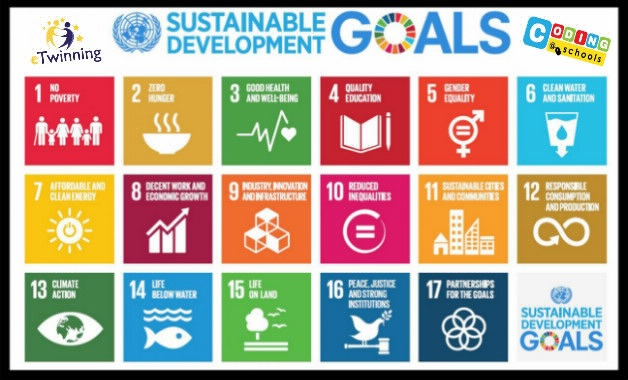
\includegraphics[width=\linewidth]{figures/SDG.png}
	\caption{Infographic illustrating the alignment of EcoCode's functionalities with the Sustainable Development Goals.}
	\label{fig:sdg_infographic}
\end{figure}

% Explanation of the workflow
\begin{figure}[H]
	\centering
	\begin{tikzpicture}[node distance=2cm]
		\node (start) [startstop] {Start};
		\node (input) [io, below of=start] {User Submits Code};
		\node (process1) [process, below of=input] {Code Analysis};
		\node (process2) [process, below of=process1] {Optimization Suggestions};
		\node (process3) [process, below of=process2] {CO2 Emission Estimation};
		\node (output) [io, below of=process3] {Display Results};
		\node (end) [startstop, below of=output] {End};

		\draw [arrow] (start) -- (input);
		\draw [arrow] (input) -- (process1);
		\draw [arrow] (process1) -- (process2);
		\draw [arrow] (process2) -- (process3);
		\draw [arrow] (process3) -- (output);
		\draw [arrow] (output) -- (end);
	\end{tikzpicture}
	\caption{Workflow of the EcoCode Application}
	\label{fig:workflow}
\end{figure}

\begin{figure}[H]
	\centering
	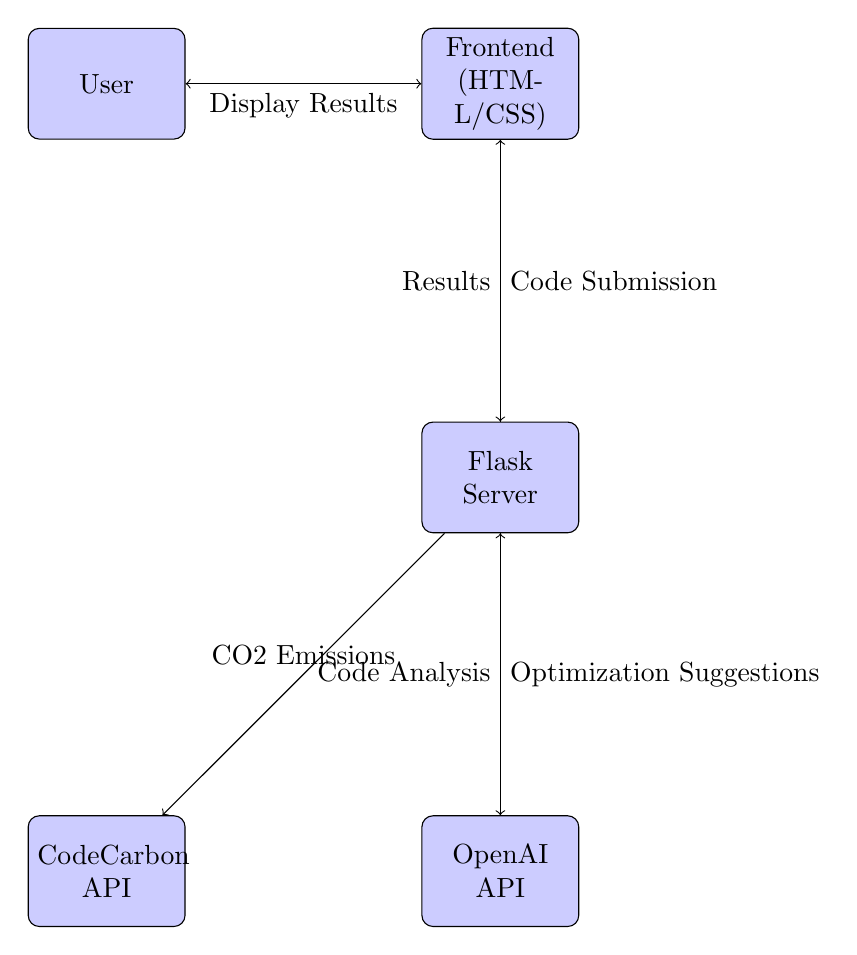
\begin{tikzpicture}[node distance=2cm, auto,
			% Define block style
			block/.style={
					rectangle,
					draw,
					fill=blue!20,
					text width=5em,
					text centered,
					rounded corners,
					minimum height=4em
				}]
		% Nodes
		\node[block] (user) {User};
		\node[block, right of=user, node distance=5cm] (frontend) {Frontend (HTML/CSS)};
		\node[block, below of=frontend, node distance=5cm] (flask) {Flask Server};
		\node[block, below of=flask, node distance=5cm] (openai) {OpenAI API};
		\node[block, left of=openai, node distance=5cm] (codecarbon) {CodeCarbon API};

		% Arrows
		\draw[->] (user) -- (frontend);
		\draw[->] (frontend) -- node {Code Submission} (flask);
		\draw[->] (flask) -- node[left] {Code Analysis} (openai);
		\draw[->] (openai) -- node[right] {Optimization Suggestions} (flask);
		\draw[->] (flask) -- node[above] {CO2 Emissions} (codecarbon);
		\draw[->] (flask) -- node[left] {Results} (frontend);
		\draw[->] (frontend) -- node {Display Results} (user);
	\end{tikzpicture}
	\caption{High-Level System Architecture of EcoCode}
	\label{fig:system_architecture}
\end{figure}


% Discussion about performance benchmarks
\begin{figure}[H]
	\centering
	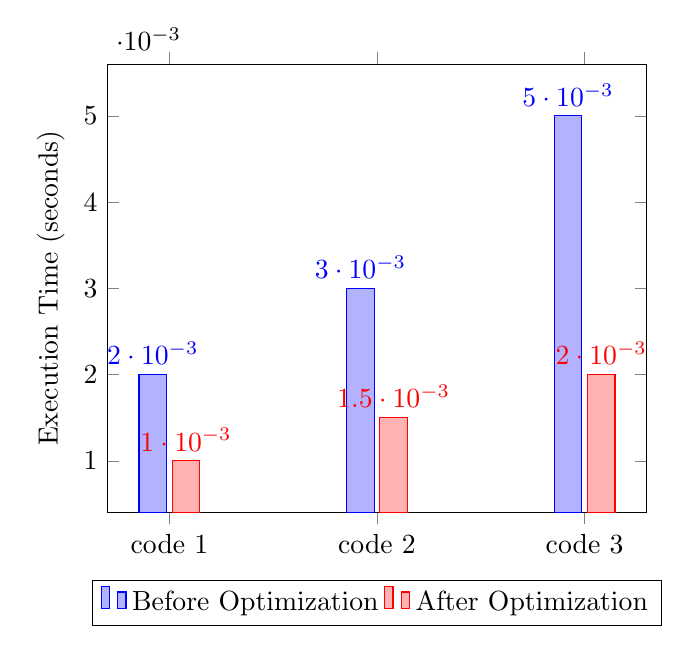
\begin{tikzpicture}
		\begin{axis}[
				ybar,
				enlargelimits=0.15,
				ylabel={Execution Time (seconds)},
				symbolic x coords={code 1, code 2, code 3},
				xtick=data,
				nodes near coords,
				nodes near coords align={vertical},
				legend style={at={(0.5,-0.15)},anchor=north,legend columns=-1},
			]

			\addplot coordinates {(code 1,0.002) (code 2,0.003) (code 3,0.005)};
			\addlegendentry{Before Optimization}

			\addplot coordinates {(code 1,0.001) (code 2,0.0015) (code 3,0.002)};
			\addlegendentry{After Optimization}

		\end{axis}
	\end{tikzpicture}
	\caption{Comparative Execution Time of codes Before and After Optimization}
	\label{fig:execution_time_comparison}
\end{figure}


\begin{figure}[H]
	\centering
	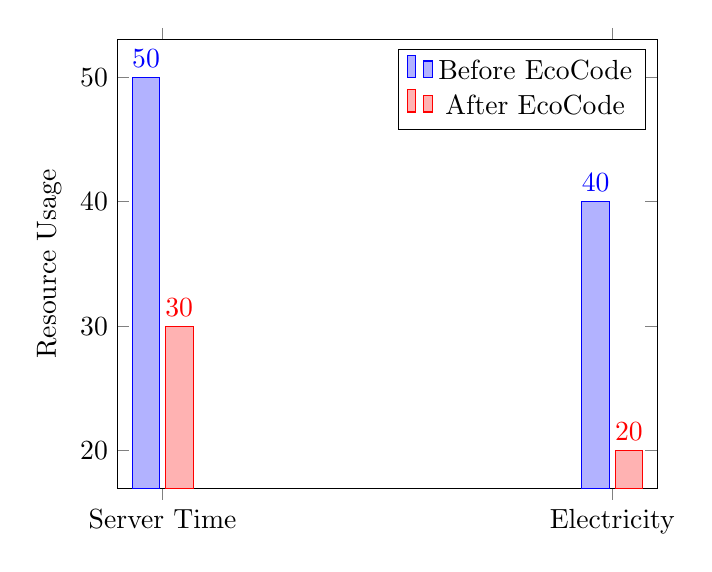
\begin{tikzpicture}
		\begin{axis}[
				ybar,
				ylabel={Resource Usage},
				symbolic x coords={Server Time, Electricity},
				xtick=data,
				nodes near coords,
				nodes near coords align={vertical},
			]
			\addplot coordinates {(Server Time, 50) (Electricity, 40)}; % Replace 50 and 40 with actual values before EcoCode
			\addplot coordinates {(Server Time, 30) (Electricity, 20)}; % Replace 30 and 20 with actual values after EcoCode
			\legend{Before EcoCode, After EcoCode}
		\end{axis}
	\end{tikzpicture}
	\caption{Comparison of resource usage before and after using EcoCode.}
	\label{fig:resource_usage}
\end{figure}


\begin{figure}[H]
	\centering
	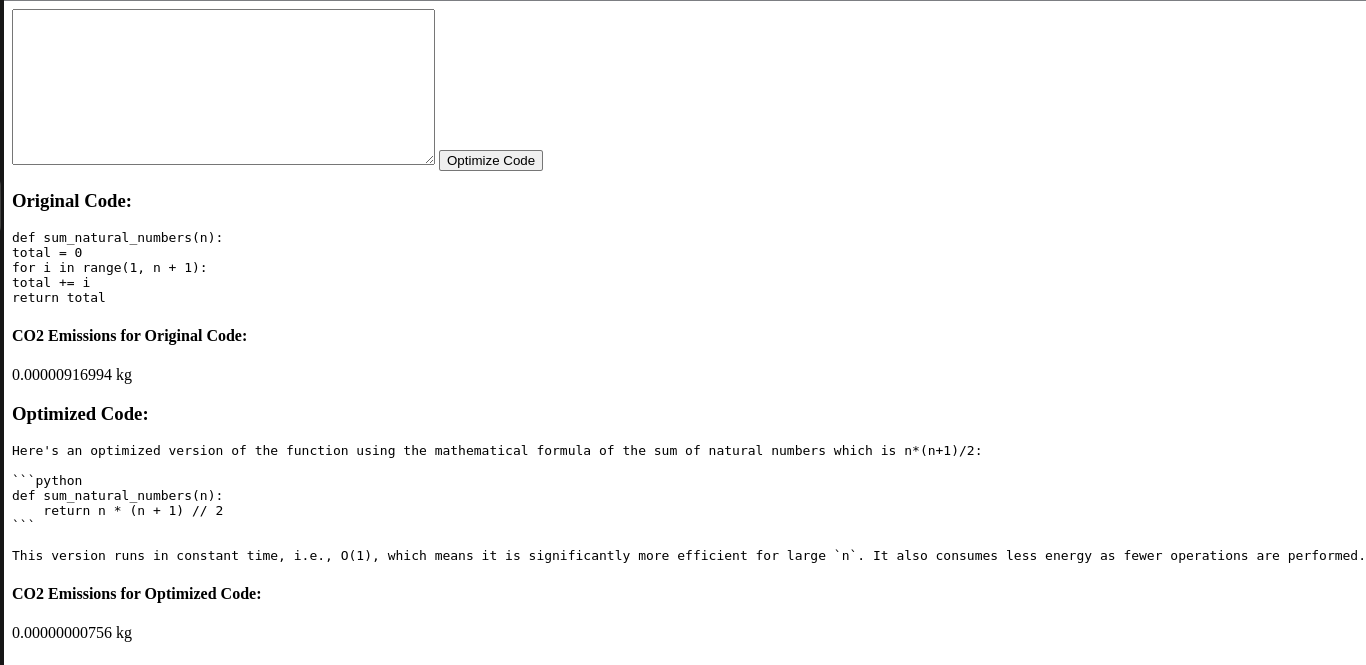
\includegraphics[width=\linewidth]{figures/Frontend.png}
	\caption{Screenshot of the EcoCode Application Frontend}
	\label{fig:frontend_screenshot}
\end{figure}

\subsection{Interaction Flow}
% Description of the interaction flow
\begin{figure}[H]
	\centering
	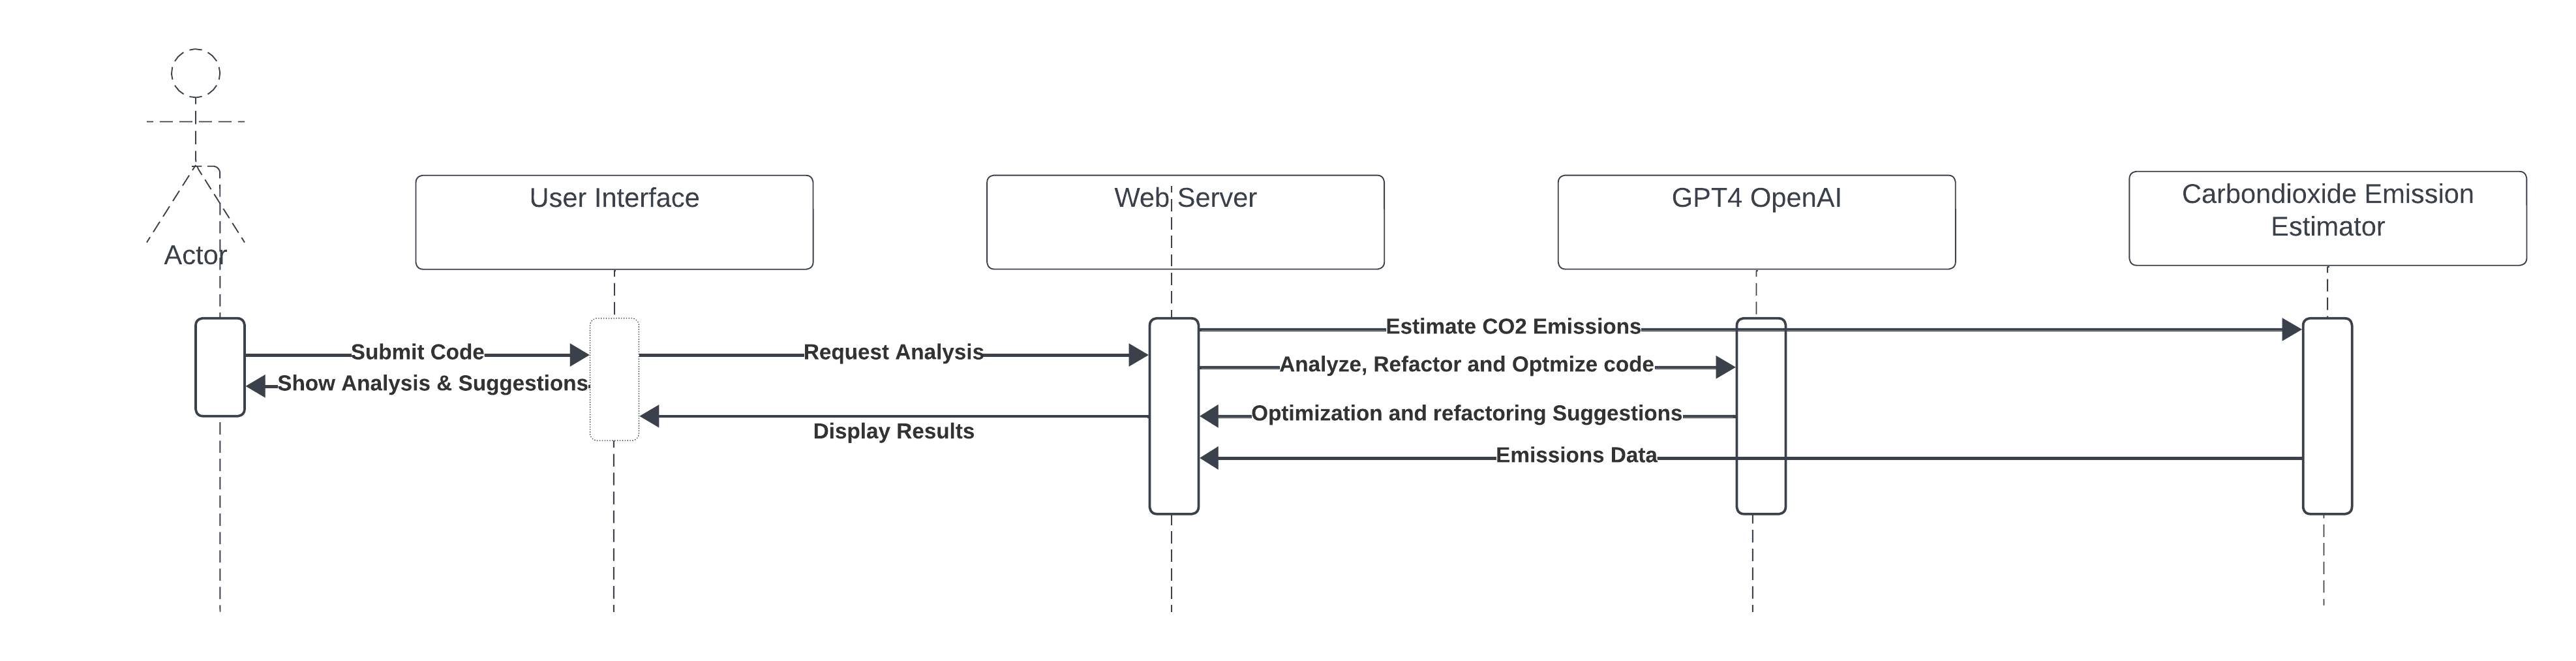
\includegraphics[width=\linewidth]{figures/Sequence Diagram.png}
	\caption{Sequence Diagram of User Interaction with EcoCode System}
	\label{fig:sequence_diagram}
\end{figure}

\section*{Plagiarism statement}
 {\it This section is mandatory to be included without modifications in the submitted report.}\\

I declare that I am aware of the following facts:
\begin{itemize}
	\item I understand that in the following statement the term "person" represents a human or \textbf{\textcolor{red}{ANY AUTOMATIC GENERATION SYTEM}}.
	\item As a student at the University of Luxembourg I must respect the rules of intellectual honesty, in particular not to resort to plagiarism, fraud or any other method that is illegal or contrary to scientific integrity.
	\item My report will be checked for plagiarism and if the plagiarism check is positive, an internal procedure will be started by my tutor. I am advised to request a pre-check by my tutor to avoid any issue.
	\item As declared in the assessment procedure of the University of Luxembourg, plagiarism is committed whenever the source of information used in an assignment, research report, paper or otherwise published/circulated piece of work is not properly acknowledged. In other words, plagiarism is the passing off as one’s own the words, ideas or work of another person, without attribution to the author. The omission of such proper acknowledgement amounts to claiming authorship for the work of another person. Plagiarism is committed regardless of the language of the original work used. Plagiarism can be deliberate or accidental.
	      Instances of plagiarism include, but are not limited to:
	      \begin{enumerate}
		      \item Not putting quotation marks around a quote from another person’s work
		      \item Pretending to paraphrase while in fact quoting
		      \item Citing incorrectly or incompletely
		      \item Failing to cite the source of a quoted or paraphrased work
		      \item Copying/reproducing sections of another person’s work without acknowledging the source
		      \item Paraphrasing another person’s work without acknowledging the source
		      \item Having another person write/author a work for oneself and submitting/publishing it (with permission, with or without compensation) in one’s own name (‘ghost-writing’)
		      \item Using another person’s unpublished work without attribution and permission (‘stealing’)
		      \item Presenting a piece of work as one’s own that contains a high proportion of quoted/copied or paraphrased text (images, graphs, etc.), even if adequately referenced
	      \end{enumerate}
	      Auto- or self-plagiarism, that is the reproduction of (portions of a) text previously written by the author without citing that text, i.e. passing previously authored text as new, may be regarded as fraud if deemed sufficiently severe.
\end{itemize}
% end-of-plagiarism section

\end{document}